\documentclass{a4beamer}
%% Lectures - common definitions

\usextensions{tikz}
\usetikzlibrary{shapes.multipart,shapes.callouts,shapes.geometric}
\input{fix-callouts.inc} % Fixes absolute positioning of rectangle callouts

\newif\ifbigpages \bigpagesfalse
\ifdim\paperwidth >20cm
	\bigpagestrue
\fi

\tikzset{%
	note/.style={rectangle callout,draw=none,callout pointer width=1em,%
		align=flush left,font=\footnotesize,inner sep=0.5em,%
		fill=blue!15,fill opacity=0.95,text opacity=1.0,callout absolute pointer=#1},
	node distance=2em and 2.75em
}
\ifbigpages
	% Scale all arrow tips by the factor of 2.5
	\let\old@pgf@arrow@call=\pgf@arrow@call
	\def\pgf@arrow@call#1{%
		\@tempdima=\pgflinewidth%
		\pgfsetlinewidth{2.5\pgflinewidth}%
		\old@pgf@arrow@call{#1}%
		\pgfsetlinewidth{\@tempdima}%
	}
	\def\pgfarrowsleftextend#1{\pgfmathsetlength{\pgf@xa}{1.5*#1}}
	\def\pgfarrowsrightextend#1{\pgfmathsetlength{\pgf@xb}{1.5*#1}}
\fi

%% Load listings package
\usepackage{listings}

%% Are we inside a comment?
\newif\iflstcomment \lstcommentfalse

\lstset{%
	tabsize=4,
	showstringspaces=false,
	basicstyle=\linespread{1.25}\ttfamily\small,
	keywordstyle=\bfseries,
	commentstyle=\lstcommentstyle,
	numbers=left,
	numberstyle=\footnotesize\color{gray},
	xleftmargin=2.5em,
	extendedchars=true,
	escapechar=\$,
	escapebegin=\iflstcomment\begingroup\lstcommentstyle\fi,
	escapeend=\iflstcomment\endgroup\fi
}

\def\lstcommentstyle{\color{gray}}

\lst@AddToHook{AfterBeginComment}{\global\lstcommenttrue}
\let\orig@lst@EndComment=\lst@EndComment
\def\lst@EndComment{\global\lstcommentfalse\orig@lst@EndComment}
\lst@AddToHookAtTop{EOL}{%
	\lst@ifLmode\global\lstcommentfalse\fi% XXX Sloppy way to determine comment end
}

%% Python with docstrings treated as comments
\lstdefinelanguage[doc]{python}[]{python}{%
	deletestring=[s]{"""}{"""},%
	morecomment=[s]{"""}{"""}%
}%

%% JavaScript language
\lstdefinelanguage{javascript}%
	{morekeywords={break,case,catch,%
		const,constructor,continue,default,do,else,false,%
		finally,for,function,if,in,instanceof,%
		new,null,prototype,%
		return,switch,this,throw,%
		true,try,typeof,var,while},%
	sensitive,%
	morecomment=[l]//,%
	morecomment=[s]{/*}{*/},%
	morestring=[b]",%
	morestring=[b]',%
}[keywords,comments,strings]%

%% C# language (4.0?)
\lstdefinelanguage{csharp}%
	{morekeywords={abstract,as,%
		base,bool,byte,case,catch,char,%
		checked,class,const,continue,%
		decimal,default,delegate,do,double,%
		else,enum,event,explicit,extern,%
		false,finally,fixed,float,for,foreach,%
		goto,if,implicit,in,int,interface,%
		internal,is,lock,long,%
		namespace,new,null,object,operator,out,%
		override,params,private,protected,public,%
		readonly,ref,return,sbyte,sealed,%
		short,sizeof,stackalloc,static,string,%
		struct,switch,this,throw,true,try,%
		typeof,uint,ulong,unchecked,unsafe,ushort,%
		using,virtual,void,volatile,while%
	},%
	sensitive,%
	morecomment=[l]//,%
	morecomment=[s]{/*}{*/},%
	morestring=[b]",%
	morestring=[b]',%
}[keywords,comments,strings]%

%% Translation for fact environment
\deftranslation[to=russian]{Fact}{Наблюдение}

%% Inline code snippets
\def\code#1{\texttt{#1}}
\def\codekw#1{\code{\textbf{#1}}}

\def\quoteauthor#1{\par\footnotesize\upshape\hfill—~#1}

%% English term
\def\engterm#1{(англ. \textit{#1})}
%% Term with explanation below (to be used in diagrams)
\def\termwithexpl#1#2{#1\strut{}\\\small\color{gray}(\textit{#2})\strut{}}
%% External link
\def\extlink#1#2{\href{#1}{\color[rgb]{0.7,0.7,1.0}\dashbar{#2}}}
%% Internal link
\def\inlink#1#2{\hyperlink{#1}{\color[rgb]{0.7,0.7,1.0}\dashbar{#2}}}
%% Explanation for a list item
\def\itemexpl#1{\begingroup\small\vspace{0.75ex}#1\par\endgroup}



\usepackage{array}


\lecturetitle{Программная инженерия. Лекция №3 — SWEBOK: основные области знаний.}
\title[SWEBOK. Основные области знаний]{SWEBOK. Основные области знаний}
\author{Алексей Островский}
\institute{\small{Физико-технический учебно-научный центр НАН Украины}\vspace{2ex}}
\date{03 октября 2014 г.}

\begin{document}
	\frame{\titlepage}
	
	\frame{
		\frametitle{Ядро знаний SWEBOK}
		
		\textbf{SWEBOK (software engineering body of knowledge)} — основной научно-технический документ по~программной инженерии, 
		отображающий знания и~накопленный опыт специалистов по~программной инженерии.
		
		\vspace{1ex}
		Ядру знаний SWEBOK соответствует стандарт ISO/IEC TR 19759:2005. 
		
		\vspace{1ex}
		\textbf{Версии:}
		\begin{itemize}
			\item
			2004 г. (SWEBOK V2) — десять областей знаний (5 основных и 5 областей управления);
			\item
			2013 г. (SWEBOK V3) — пятнадцать областей (+ теоретические основы ПИ, \\ экономика и описание профессиональных навыков по ПИ).
		\end{itemize}
	}
	
	\frame{
		\frametitle{Основные области знаний SWEBOK}
		
		\def\areamember#1{\small\color{gray}#1\strut{}}
\linespread{1.0}
\begin{tikz*}[
	every node/.style={draw,rectangle split,rectangle split parts=2,align=center}
]
	\node(areas) [rectangle,minimum width=35em] {\large Основные области знаний SWEBOK\strut{}};

	\node(design) [above=1em of areas] {
		\textbf{Проектирование ПО}
		\nodepart{two}
		\areamember{базовые концепции} \\ 
		\areamember{ключевые вопросы} \\
		\areamember{архитектура} \\
		\areamember{нотации} \\ 
		\areamember{стратегия и методы}
	};
	\node(req) [left=2em of design.south west,anchor=south east] {
		\textbf{Инженерия требований}
		\nodepart{two}
		\areamember{определение} \\ 
		\areamember{анализ} \\ 
		\areamember{спецификация} \\ 
		\areamember{проверка} \\ 
		\areamember{управление}
	};
	\node(construct) [right=2em of design.south east,anchor=south west] {
		\textbf{Конструирование ПО}
		\nodepart{two}
		\areamember{снижение сложности} \\ 
		\areamember{ориентация на изменения} \\ 
		\areamember{валидация} \\ 
		\areamember{внешние стандарты} \\
		\areamember{}
	};

	\node(_tmp) at (areas.south -| req.east) [coordinate]{};
	\node(testing) [below=1em of _tmp,anchor=north] {
		\textbf{Тестирование ПО}
		\nodepart{two}
		\areamember{концепции} \\ 
		\areamember{уровни тестирования} \\ 
		\areamember{техники} \\ 
		\areamember{метрики} \\ 
		\areamember{управление тестированием}
	};
	\node(_tmp) at (areas.south -| construct.west) [coordinate]{};
	\node(maintenance) [below=1em of _tmp,anchor=north] {
		\textbf{Сопровождение ПО}
		\nodepart{two}
		\areamember{концепции} \\ 
		\areamember{сопровождение} \\ 
		\areamember{ключевые вопросы} \\ 
		\areamember{спецификация требований} \\ 
		\areamember{процесс сопровождения}
	};
	
	\draw[->] (areas.north -| req.south) to (req.south);
	\draw[->] (areas) to (design);
	\draw[->] (areas.north -| construct.south) to (construct.south);
	\draw[->] (areas.south -| testing.north) to (testing.north);
	\draw[->] (areas.south -| maintenance.north) to (maintenance.north);
\end{tikz*}

	}
	
	\section{Требования}
	
	\subsection{Определение}
	
	\frame{
		\frametitle{Требования к ПО}
		
		\begin{Definition}
			\textbf{Требование к программному обеспечению} \engterm{software requirement} — это:
			\begin{itemize}
				\item
				характеристика ПО, с помощью которой конечным пользователем ПО решается какая-либо задача или достигается определенная цель;
				\item
				характеристика или свойство ПО, определенное контрактом на его разработку или~другим документом (стандартом, спецификацией и т.\,п.).
			\end{itemize}
		\end{Definition}

		\vspace{1ex}
		\textbf{Цель требований:}
		\begin{itemize}
			\item
			определение функций, условий и~ограничений, присущих~ПО; 
			\item
			спецификация данных, технического сопровождения и~среды исполнения.
		\end{itemize}
	}

	\subsection{Виды требований}
	
	\frame{	
		\frametitle{Виды требований}

		\begin{itemize}
			\item
			\textbf{Требования к продукту и процессу} — условия выполнения и~режим работы~ПО, 
			ограничения на~среду исполнения; определение принципов взаимодействия
			с~другими~программами.

			\vspace{1ex}
			\item
			\textbf{Функциональные требования} — определяют назначение и~функции системы.

			\vspace{1ex}
			\item
			\textbf{Нефункциональные требования} — определяют условия исполнения~ПО, 
			переносимости и~доступа к~данным.

			\vspace{1ex}
			\item
			\textbf{Системные требования} — требования к~программной системе в~целом.
		\end{itemize}
	}

	\subsection{Инженерия требований}
	
	\frame{
		\frametitle{Инженерия требований}

		\begin{Definition}
			\textbf{Инженерия требований} \engterm{requirements engineering} — процесс формулировки, документирования 
			и~поддержки требований к~ПО, а~также соответствующая область программной инженерии.
		\end{Definition}
		
		\begin{figure}
			{\small\begin{tikz*}[%
	every node/.style={rectangle,align=center,minimum height=3em},
	node distance=2em and 2em
]
	\node(req) {\textbf{Инженерия} \\ \textbf{требований}};
	\node(design) [right=of req] {Проектирование};
	\node(construct) [right=of design] {Конструирование};
	\node(testing) [right=of construct] {Тестирование};
	\node(maint) [right=of testing] {Сопровождение};
	
	\draw[->] (req) to (design);
	\draw[->] (design) to (construct);
	\draw[->] (construct) to (testing);
	\draw[->] (testing) to (maint);
\end{tikz*}
}
			\caption{В классической модели жизненного цикла \engterm{waterfall model} инженерия требований — начальный процесс разработки~ПО.}
		\end{figure}

		\begin{figure}
			{\small\begin{tikz*}[%
	every node/.style={rectangle,align=center,minimum height=2.5em},
	node distance=2em and 2em
]
	\node(req) at (0, 0) {\textbf{Инженерия} \\ \textbf{требований}};
	\node(design) [right=of req] {Проектирование};
	\node(construct) [right=of design] {Констр.};
	\node(testing) [right=of construct] {Тестирование};
	\node(maint) [right=of testing] {Сопровождение};
	
	\draw[->] (req) to (design);
	\draw[->] (design) to (construct);
	\draw[->] (construct) to (testing);
	\draw[->] (testing) to (maint);
	
	\draw (design) -- ++(0,-3em);
	\draw (construct) -- ++(0,-3em);
	\draw (testing) -- ++(0,-3em);
	\draw[->] (maint) -- ++(0,-3em) -| (req);
\end{tikz*}
}
			\caption{В других моделях (RUP, extreme programming, Scrum) требования уточняются в процессе разработки.}
		\end{figure}
	}
	
	\frame{
		\frametitle{Составляющие инженерии требований}
		
		\vspace*{5ex}
		\begin{overlayarea}{\textwidth}{0.6\textheight}
			{\small\begin{tikz*}[%
	iteration/.style={rectangle,align=center}
]
	\node[iteration] (elic) {
		\termwithexpl{определение}{elicitation}
	};
	\node[iteration,right=of elic] (analysis) {
		\termwithexpl{анализ}{analysis}
	};
	\node[iteration,right=of analysis] (spec) {
		\termwithexpl{спецификация}{specification}
	};
	\node[iteration,right=of spec] (valid) {
		\termwithexpl{проверка}{validation}
	};
	\node[iteration,right=of valid] (manage) {
		\termwithexpl{управление}{management}
	};
	
	\draw[->] (elic) to (analysis);
	\draw[->] (analysis) to (spec);
	\draw[->] (spec) to (valid);
	\draw[->] (valid) to (manage);
\end{tikz*}
}
		\end{overlayarea}
	}
	
	\section{Проектирование}
	
	\subsection{Определение}
	
	\frame{
		\frametitle{Проектирование программного обеспечения}

		\begin{Definition}
			\textbf{Проектирование ПО} \engterm{software design} — процесс определения архитектуры~ПО, 
			набора составляющих компонентов и~их~интерфейсов, прочих характеристик системы и~конечного состава программного продукта.
		\end{Definition}

		\vspace{1ex}
		Основные \textbf{концепции} проектирования ПО:
		\begin{itemize}
			\item
			\textbf{абстрагирование} (отсеивание лишней информации) и~\textbf{уточнение} 
			(построение иерархии выполнения);
			\item
			\textbf{модульность} (выделение автономных компонентов системы) и~\textbf{архитектура} \\
			(общая структура системы, связывающая все~компоненты);
			\item
			\textbf{структуризация} (представления взаимоотношений между данными) и~\textbf{инкапусляция} 
			(отделение реализации от~представления).
		\end{itemize}
	}
	
	\subsection{Архитектура ПО}
	
	\frame{
		\frametitle{Архитектура ПО}

		\begin{Definition}
			\textbf{Архитектура программного проекта} — высокоуровневое представление структуры системы 
			и~спецификация ее~компонентов и~логики их~взаимодействия.
		\end{Definition}

		\vspace{1ex}
		\textbf{Преимущества} использования архитектуры ПО:
		\begin{itemize}
			\item основа для~анализа системы на~ранних этапах ее~разработки;
			\item основа для~повторного использования компонентов и~решений;
			\item упрощение принятия решений касательно разработки, развертывания и~поддержки~ПО;
			\item упрощение диалога с~заказчиком;
			\item уменьшение рисков и~снижение затрат на~производство~ПО.
		\end{itemize}
	}
	
	\subsection{Шаблоны проектирования}

	\frame{
		\frametitle{Шаблоны проектирования}

		\begin{Definition}
		\textbf{Шаблон проектирования} \engterm{design pattern} — типовой конструктивный элемент программной системы, 
		задающий взаимодействие нескольких компонентов системы, а~также роли и~сферы ответственности исполнителей. 
		\end{Definition}

		\vspace{1ex}
		\textbf{Виды шаблонов}:
		\begin{itemize}
			\item
			порождающие \engterm{creational patterns} — связанные с~созданием объектов. \\
			\textbf{Пример:} фабрика (\extlink{http://en.wikipedia.org/wiki/Factory_method_pattern}{factory}), 
			синглтон (\extlink{http://en.wikipedia.org/wiki/Singleton_pattern}{singleton}).

			\item
			структурные \engterm{structural patterns} — определяющие структуру композиции из~нескольких объектов. \\
			\textbf{Пример:} мост (\extlink{http://en.wikipedia.org/wiki/Bridge_pattern}{bridge}), 
			декоратор (\extlink{http://en.wikipedia.org/wiki/Decorator_pattern}{decorator}).

			\item
			поведенческие \engterm{behavioral patterns} — определяющие поведение объектов. \\
			\textbf{Пример:} итератор (\extlink{http://en.wikipedia.org/wiki/Iterator_pattern}{iterator}). 
		\end{itemize}
	}
	
	\subsection{Инструменты проектирования}

	\frame{
		\frametitle{Инструменты проектирования}

		Описание элементов ПО осуществляется с помощью \textbf{нотаций проектирования}.

		\vspace{1ex}
		\begin{overlayarea}{\textwidth}{0.72\textheight}
			\only<1>{
				\textbf{Структурная нотация} — представление основных аспектов элементов ПО, их~интерфейсов и~взаимосвязей. 

				\vspace{1ex}
				\begin{columns}
					\begin{column}{0.47\textwidth}
						\begin{figure}
							
\includegraphics[width=\textwidth]{decorator.png}\vspace{-2ex}
							\caption{UML-описание шаблона «Декоратор»}
						\end{figure}
					\end{column}
					\begin{column}{0.5\textwidth}
						\textbf{Инструменты:} 
						\begin{itemize}
							\item ADL (architecture description language);
							\item UML (unified modeling language); 
							\item ERD (entity – relation diagrams);
							\item IDL (interface description language).
						\end{itemize}
					\end{column}
				\end{columns}
			}
			\only<2>{
				\textbf{Поведенческая нотация} — определенное представление динамики работы системы и~ее~элементов. 
				
				\vspace{1ex}
				\begin{columns}
					\begin{column}{0.35\textwidth}
						\begin{figure}
							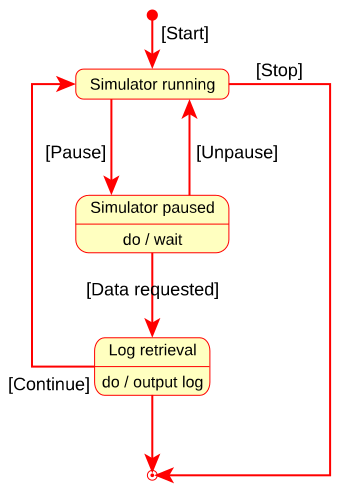
\includegraphics[width=0.8\textwidth]{state-diagram.png}\vspace{-2ex}
							\caption{Диаграмма состояний эмулятора}
						\end{figure}
					\end{column}
					\begin{column}{0.63\textwidth}
						\textbf{Инструменты:} 
						\begin{itemize}
							\item диаграммы потоков данных (data flow);
							\item таблицы принятия решений (decision tables);
							\item формальные языки спецификации (Z, VDM, RAISE).
						\end{itemize}
					\end{column}
				\end{columns}
			}
		\end{overlayarea}
	}

	\section{Конструирование}
	
	\subsection{Определение}
	
	\frame{
		\frametitle{Конструирование ПО}

		\begin{Definition}
			\textbf{Конструирование ПО} \engterm{software construction} — создание~ПО из~составных элементов (блоков, операторов, функций) 
			и его проверка методами верификации и~тестирования.
		\end{Definition}

		\vspace{1ex}
		\textbf{Техники конструирования:}
		\begin{itemize}
			\item кодирование;
			\item верификация, модульное тестирование (unit testing), 
			тестирование итеграции (integration testing);
			\item отладка (debugging).
		\end{itemize}

		\vspace{1ex}
		\textbf{Инструменты конструирования:}
		\begin{itemize}
			\item
			языки конструирования; 
			\item
			программные методы и~инструментальные системы 
			(компиляторы, СУБД, генераторы отчетов, системы управления конфигурацией).
		\end{itemize}
	}

	\frame{
		\frametitle{Основы конструирования ПО}

		\begin{itemize}
			\item
			\textbf{Снижение сложности} \engterm{minimizing complexity} — акцент на~читаемости кода, а~не~его~«красоте». 
			Keep~it simple, stupid (KISS).

			\vspace{0.5ex}
			\textbf{Средства достижения:} стандарты кодирования.

			\vspace{0.5ex}
			\item
			\textbf{Ожидание изменений} \engterm{anticipating change} — использование инструментов, 
			позволяющих оперативно вносить изменения и~дополнять код.

			\vspace{0.5ex}
			\textbf{Средства достижения:} средства коммуникации (напр., системы документирования), диаграммы UML.

			\vspace{0.5ex}
			\item
			\textbf{Структуризация для проверок} \engterm{constructing for verification} — построение ПО, 
			ошибки в~котором выявляются на~как~можно более ранних этапах.

			\vspace{0.5ex}
			\textbf{Средства достижения:} обзоры кода (code reviews), модульное тестирование, автоматизация тестирования.
		\end{itemize}
	}

	\subsection{Стандарты при конструировании}
	
	\frame{
		\frametitle{Стандарты при конструировании}
		
		{\small\begin{tikz*}[%
	every node/.style={rectangle,align=center,minimum height=2em}
]
	\node[inner sep=0.5em] (st) {\textbf{Стандарты конструирования ПО}};
	\node[inner sep=0.5em,above=of st] (ext) {Внешние стандарты};
	\node[above=of ext] (pl) {\termwithexpl{Языки программирования}{Java, C++, C\#, Python, …}};
	\node[left=of pl] (dl) {\termwithexpl{Языки описания данных}{XML, SQL, YAML, …}};
	\node[right=of pl] (il) {\termwithexpl{Интерфейсные языки}{IDL, UML, …}};
	\node[below=of dl] (api) {\termwithexpl{Интерфейсы ОС}{API}};
	\node[right=of ext] (inter) {\termwithexpl{Стандарты взаимодействия}{COM, CORBA, …}};
	
	\node[inner sep=0.5em,below=of st] (int) {Внутренние стандарты};
	\node[below left=of int] (team) {Координация групповой \\ деятельности};
	\node[below=of int] (gen) {Общие стандарты};
	\node[below right=of gen] (verify) {Структуризация \\ для проверок};
	\node[left=of verify] (change) {Ожидание \\ изменений};
	\node[left=of change] (compl) {Снижение \\ сложности};

	\draw[->] (st) to (ext);
	\draw[->] (ext) to (pl);
	\draw[->] (ext) to (dl);
	\draw[->] (ext) to (il);
	\draw[->] (ext) to (api);
	\draw[->] (ext) to (inter);
	
	\draw[->] (st) to (int);
	\draw[->] (int) to (team);
	\draw[->] (int) to (gen);
	\draw[->] (gen) to (compl);
	\draw[->] (gen) to (change);
	\draw[->] (gen) to (verify);
\end{tikz*}
}
	}

	\subsection{Управление конструированием}
	
	\frame{
		\frametitle{Управление конструированием}

		\begin{Definition}
			\textbf{Управление конструированием} \engterm{managing construction} — управление процессом конструирования ПО, включающим в себя следующие этапы:
			\begin{enumerate}
				\item
				создание модели конструирования, зависящей от выбранной модели жизненного цикла ПО;
				\item
				планирование конструирования — определение расписания конструкторских работ и~их~распределения между исполнителями;
				\item
				измерение показателей — выработка количественных показателей (напр., объем нового / повторно использованного кода; 
				сложность кода; число обнаруженных / исправленных ошибок) для корректировки процесса разработки.
			\end{enumerate}
		\end{Definition}
	}

	\section{Тестирование}
	
	\subsection{Определение}
	
	\frame{
		\frametitle{Тестирование ПО}

		\begin{Definition}
			\textbf{Тестирование ПО} — это процесс проверки готовой программы в~\emph{статике} (обзоры кода, инспекции и~т.\,п.) 
			и~\emph{динамике} (прогон программы на~тестовых данных) с~целью обеспечить ее~соответствие заданным требованиям.
		\end{Definition}

		\vspace{1ex}
		\textbf{Виды тестирования:} 
		\begin{itemize}
			\item модульное (unit testing);
			\item интеграционное (integration testing);
			\item системное (system testing);
			\item приемка (acceptance testing).
		\end{itemize}
	}
	
	\frame{
		\frametitle{Основные понятия тестирования}

		\textbf{Этапы возникновения сбоев} в программе:
		\begin{enumerate}
			\item
			программист совершает \emph{ошибку} (error, mistake);
			\item
			ошибка приводит к \emph{дефекту} (defect, fault, bug) в исходном коде;
			\item
			при определенных условиях исполнения дефект приводит к \emph{сбою программы} (program failure).
		\end{enumerate}

		\vspace{1ex}
		\textbf{Тест} — набор входных данных и прочих условий (напр., характеристики операционной системы и оборудования), 
		которые полностью определяют ход выполнения программы.

		\vspace{1ex}
		\textbf{Цель тестирования} — локализация и устранение дефектов, соответствующие всем сбоям программы, 
		обнаруженным с помощью тестов.

		\vspace{2ex}
		{\linespread{1.0}\begin{tikz*}[every node/.style={rectangle,align=center}]
			\node (all) at (0, 0) {
				Прогон \emph{всех} тестов невозможен \\
				даже для простых систем.
			};
			\node[right=of all] (imply) {
				\Large $\Rightarrow$
			};
			\node[right=of imply] (info) {
				Необходим отбор \\
				\emph{информативных} тестов.
			};
		\end{tikz*}}
	}
	
	\subsection{Методы тестирования}
	
	\frame{
		\frametitle{Методы тестирования}

		\begin{itemize}
			\item
			\textbf{Белый ящик} \engterm{white box testing}, структурное тестирование 
			— тестирование внутренних структур и операций ПО.

			\vspace{0.5ex}
			\textbf{Виды:} тестирование API, внедрение ошибок (fault injection), покрытие кода (code coverage), 
			мутационное тестирование (mutation testing), статическое тестирование (static testing).

			\vspace{0.5ex}
			\item
			\textbf{Черный ящик} \engterm{black box testing} — тестирование функциональности, доступной конечному пользователю ПО.

			\vspace{0.5ex}
			\textbf{Виды:} анализ граничных значений (boundary value analysis), таблицы принятия решений (decision table testing), 
			тестирование прецедентов (use case testing), тестирование потоков данных (data flow testing) и~т.\,д.

			\vspace{0.5ex}
			\item
			\textbf{Серый ящик} \engterm{gray box testing} — тестирование ПО с~частичным знанием о~его~внутренней структуре.

			\vspace{0.5ex}
			\textbf{Виды:} тестирование интерфейсов компонентов системы, анализ обработки ошибок и~т.\,п.
		\end{itemize}
	}
	
	\subsection{Типы тестирования}
	
	\frame{
		\frametitle{Типы тестирования}

		\begin{itemize}
			\item
			\textbf{тестирование установки} ПО;
			\item
			\textbf{тестирование совместимости} (напр., с операционной системой и оборудованием);
			\item
			\textbf{проверка работоспособности} \engterm{sanity check} — проверка на отсутствие тривиальных ошибок;
			\item
			\textbf{функциональное тестирование} — проверка реализации функций ПО, определенных в~требованиях, и корректности их исполнения;
			\item
			\textbf{регрессионное тестирование} — повторная проверка функциональности ПО после внесения значительных изменений;
		\end{itemize}
	}
	
	\frame{
		\frametitle{Типы тестирования (продолжение)}

		\begin{itemize}
			\item
			\textbf{тестирование эффективности} — проверка скорости исполнения, продуктивности, используемого объема памяти и т.\,п.;
			\item
			\textbf{стресс-тестирование} — проверка поведения системы при превышении допустимой нагрузки;
			\item
			\textbf{альфа-} и \textbf{бета-тестирование} — тестирование системы тестировщиками разработчика (альфа) 
			и ограниченной группой сторонних пользователей (бета);
			\item
			\textbf{тестирование безопасности};
			\item
			\textbf{тестирование интерфейса} ПО, usability, локализации и т.\,д.
		\end{itemize}
	}

	\subsection{Управление тестированием}
	
	\frame{
		\frametitle{Управление тестированием}

		\textbf{Основные этапы тестирования:}
		\begin{enumerate}
			\item
			планирование процесса тестирования, составление планов, тестов, наборов данных;
			\item
			проведение тестирования компонентов повторного использования и шаблонов;
			\item
			генерация тестовых сценариев, соответствующих среде выполнения ПО;
			\item
			сбор сведений об отказах ПО и выявленных исключительных ситуациях;
			\item
			подготовка отчетов о результатах тестирования и оценка характеристик системы.
		\end{enumerate}
	}

	\section{Сопровождение}
	
	\subsection{Определение}
	
	\frame{
		\frametitle{Сопровождение ПО}

		\begin{Definition}
			\textbf{Сопровождение ПО} \engterm{software maintenance} — совокупность действий по~обеспечению работы ПО, 
			внесению изменений при~выявлении ошибок, адаптации к~новой среде исполнения, улучшения продуктивности или~других характеристик ПО.
		\end{Definition}

		\vspace{1ex}
		\textbf{Основные вопросы} сопровождения ПО: 
		\begin{itemize}
			\item
			технические вопросы (напр., тестирование, анализ изменений); 
			\item
			вопросы управления (напр., организация персонала); 
			\item
			экономические вопросы (оценка стоимости сопровождения); 
			\item
			измерительные вопросы (создание метрик для анализа эффективности сопровождения).
		\end{itemize}
	}
	
	\subsection{Категории сопровождения}
	
	\frame{
		\frametitle{Категории сопровождения}

		\begin{center}
			\begin{tabular}{|*{3}{p{0.25\textwidth}|}}
				\hline
				\centering По времени & \multicolumn{2}{c|}{По наличию ошибки} \\
				\cline{2-3}
				& \centering исправление & \centering совершенствование \cr
				\hline
				упреждающее & \centering предотвращение & \centering улучшение \cr
				\hline
				ответное & \centering корректировка & \centering адаптация \cr
				\hline
			\end{tabular}
		\end{center}

		\vspace{1ex}
		\begin{itemize}
			\item
			\textbf{корректировка} — устранение выявленных ошибок или нереализованных требований;
			\item
			\textbf{адаптация} — настройка продукта к изменившимся условиям эксплуатации;
			\item
			\textbf{предотвращение ошибок} — устранение скрытых дефектов, которые потенциально могут привести к~сбоям;
			\item
			\textbf{улучшение} — увеличение продуктивности или повышение уровня сопровождения.
		\end{itemize}
	}

	\subsection{Методики сопровождения}
	
	\frame{
		\frametitle{Методики сопровождения ПО}

		\begin{itemize}
			\item
			\textbf{Понимание программ} \engterm{program comprehension} — чтение и осмысление кода~ПО с~целью внесения в него изменений.
			\item
			\textbf{Реинженерия} \engterm{reengineering} — усовершенствование ПО путем реорганизации или реструктуризации, 
			а~также настройка параметров и~программных элементов для новой среды исполнения.
			\item
			\textbf{Реверсная инженерия} \engterm{reverse engineering} — анализ ПО для выделения его~компонент и взаимоотношений между ними.

			Используется для создания абстрактного представления ПО, чаще всего для~перепрограммирования ПО для~новой среды исполнения.
			\item
			\textbf{Рефакторинг} \engterm{refactoring} — реорганизация кода программы для улучшения ее~структуры, не изменяющая функциональность ПО.
		\end{itemize}
	}

	\section{Заключение}
	
	\subsection{Выводы}

	\frame{
		\frametitle{Выводы}

		\begin{enumerate}
			\item
			Ядро SWEBOK содержит пять основных областей знаний программной инженерии 
			(инженерия требований, проектирование, конструирование, тестирование и~сопровождение ПО), 
			которые соответствуют процессам жизненного цикла ПО.

			\vspace{0.5ex}
			\item
			Основные области знаний содержат в~себе как \emph{теоретические основы}, 
			так~и~систематизированные \emph{практические навыки} разработки ПО, 
			а~также \emph{методы управления} процессами разработки.

			\vspace{0.5ex}
			\item
			Все пять основных процессов ЖЦ тесно связаны между собой; особенности их~взаимодействия 
			сильно зависят от~выбранной модели жизненного цикла.
		\end{enumerate}
	}

	\subsection{Материалы}
	
	\frame{
		\frametitle{Материалы}
		
		\begin{thebibliography}{9}
			\bibitem[1]{1}
			Лавріщева К.\,М. 
			\newblock Програмна інженерія (підручник). 
			\newblock {\footnotesize К., 2008. — 319 с.}

			\bibitem[2]{2}
			Описание стандарта SWEBOK.
			\newblock {\footnotesize\url{http://www.computer.org/portal/web/swebok/html/contents}}
		\end{thebibliography}
	}
	
	\frame{
		\frametitle{}
		
		\begin{center}
			\Huge Спасибо за внимание!
		\end{center}
	}
\end{document}
